\newpage
\section{Theorie}
\label{sec:theorie}
Ziel: Bestimmung der Dampfdruckkurve im Bereich ca. 30-1000mbar.
Zusätzlich soll die zugehörigen Verdampfungswärme $L$ und dessen temperaturabhängigkeit bestimmt werden.\\

\subsection{Mikroskopische Vorgänge}
In einer Flüssigkeit bewegen sich die Teilchen mit der Maxwell'schen Geschwindigkeitsverteilung.
Einige Moleküle haben genug kinetische Energie um die Flüssigkeit zu verlassen.
Dabei verrichten sie Arbeit, dessen Energie von außen durch z.B. das Erhitzen hinzugefügt werden muss.
Die Moleküle die wieder auf die Flüssigkeitsoberfläche treffen, können von dieser wieder eingefangen werden.
Nach einer gewissen Zeit stellt sich ein Gleichgewicht ein zwischen den Molekülen die die Flüssigkeit verlassen und deren
die wieder eingefangen werden.
Es stellt sich ein konstanter Druck (genannt Sättigungsdruck) ein, dieser ist Gasraum-Volumen unabhängig. 
Der Vorgang der Verdampfung ist zu diesem Zeitpunkt beendet und
die Flüssigkeit und der Dampf koexistiert.\\
Das Verhalten des gesättigen Dampfes entspricht der Allgemeinen Gasgleichung:
\begin{equation}
    pV=RT
    \label{eqn:gasgl}
\end{equation}
wobei R die Allgemeine Gaskonstante ist.

\begin{figure}
    \centering
    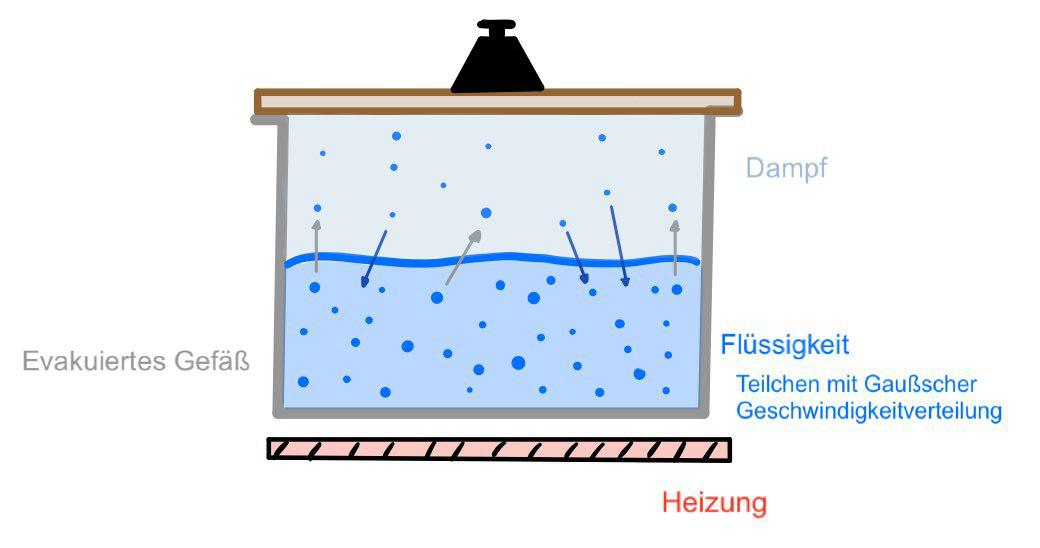
\includegraphics[width=0.7\textwidth]{bilder/kessel.jpg}
    \caption{Druckkessel}
    \label{fig:kessel}
\end{figure}

Betrachtet wird der Phasenübergang von Wasser.
Dabei haben generell die Phasen (fest, flüssig, gasförmig) zwei Freiheitsgerade - die Temperatur $T$ und den Druck $p$.
Dabei gibt es Bereiche in denen zwei Phasen nebeneinander vorliegen. Hierbei sind die Termperaturen $T$ und der Druck $p$
nicht frei wähltbar. Es liegt nur noch ein Freiheitsgrad vor.\\
Diese Bereiche werden durch die Dampfdruck-Kurve beschrieben, die die Phasen von einander abgrenzt.
Auf dieser Kurve gibt es zwei charakteristische Punkt:
\begin{figure}
    \centering
    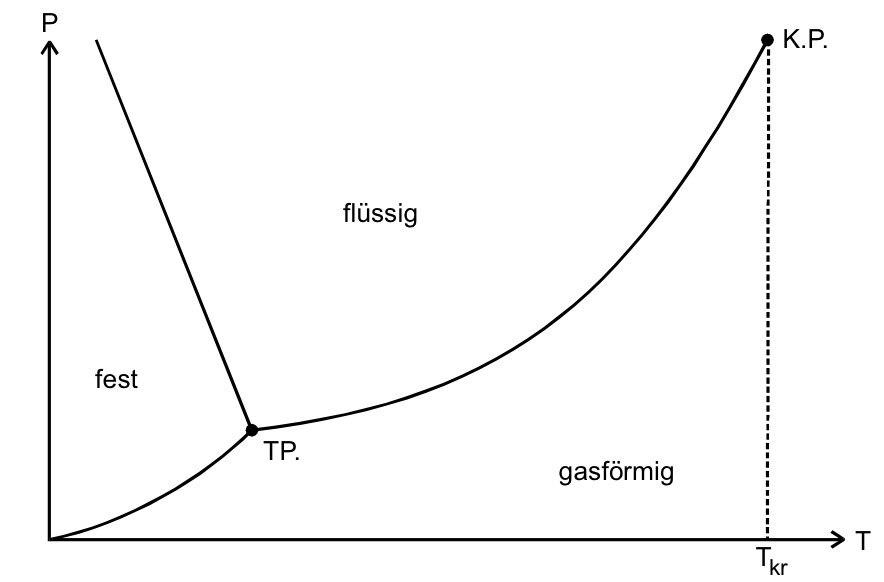
\includegraphics[width=0.5\textwidth]{bilder/zustandsdiagramm.jpg}
    \caption{Zustandsdiagramm des Wassers \cite[176]{Anleitung}}
    \label{fig:diagramm}
\end{figure}
\newpage
\begin{enumerate}
    \item Trippel-Punkt (T.P.): Beschreibt den Zustand in denen alle drei Aggregardszustände neben einander vorliegen.
    \item Kritischer Punkt (K.P.): Ist das Ende der Dampfdruckkurve, und beschreibt den Zustand in dem es keinen Unterschied
        zwischen dem Aggregatszustand flüssig und gasförmig nicht mehr unterchieden werden kann.
\end{enumerate}
Befindet man sich irgendwo anders auf der Kruve, so koexistieren zwei Phasen.
\subsection{Verdampfungswärme $L$}
Die Dampfdruckkurve wird bestimmt durch die Verdampfungswärme $L$.
Diese Größe ist eine charakteristische Größe der Substanz und im allgemeinen temperaturabhängig.
Allerdings verhält sie sich in Nähe des Trippel Punktes in guter Näherung konstant (temperaturunabhängig).\\\newline
\uline{Definition molare Verdampfungswärme $L$:}
\begin{flushleft}
Gibt die Enerie an, die benötigt wird um einen Mol einer Flüssigkeit in Dampf der
der gleichen Temperatur umzuwandeln.
\end{flushleft}

\subsection{Clausius-Clapeyronsche Gleichung}
Liegt die Temperatur $T$ weit unter dem kritischen Punkt K.P., so gelten folgende Näherungen:
\begin{enumerate}
    \item Das Volumen der Flüssigkeit $V_F$ ist gegenüber dem Volumen des Dampfes $V_D$ vernachlässigbar
    \item $V_D$ lässt sich durch die Allgemeine Gasgleichung \ref{eqn:gasgl} beschreiben
    \item $L$ ist druck- und temperaturunabhängig
    \begin{equation}
        \frac{R}{p}\;dp=\frac{L}{T^2}\;dT
    \end{equation}
\end{enumerate}
somit folgt:
\begin{equation}
    (V_D-V_F)\;dp=\frac{L}{T}\;dT
    \label{eqn:L}
\end{equation}
Dabei können $V_D$ und $V_F$ komplizierte Funktionen der Temperatur $T$ sein, wodurch eine 
Integration im allgemeinen schwierig ist.\\
Unter den angeführten Bedingungen folgt aber für die Integration:
\begin{gather}
    \textrm{ln($p$)} = -\frac{L}{R}\;\frac{1}{T}+\textrm{const}
   \Longleftrightarrow p=p_0\;exp(-\frac{L}{R}\cdot \frac{1}{T})
   \label{eqn:logarithm_p}
\end{gather}